\section{User experience goals}\textit{Dennis}\\
The user should not find this system specially emotional or fun as the system might be seen as frivolous if it is overdone. However, to keep the interest of the visitors (primarily high school students), the system should be entertaining to a certain level.  
Down below the different user experience goals are listed in order (so most important at the top):
\begin{enumerate}
	\item Rewarding
	\item Helpful
	\item Entertaining
	\item Motivating
	\item Enjoyable
	\item Fun
	\item Satisfying
	\item Aesthetically pleasing
	\item Emotionally fulfilling
\end{enumerate}


\begin{wrapfigure}{r}{0.4\textwidth}
	\center
		\setlength\fboxsep{0pt}
		\setlength\fboxrule{0pt}
		\fbox{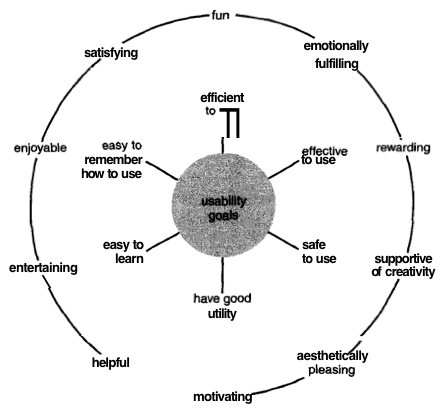
\includegraphics[width=0.4\textwidth]{images/usability_goals_diagram.png}}
   	\caption{\textit{The difference between usability and user experience goals, where  usability goals are central to
  			interaction design and are operationalized through specific criteria. 
  			User experience goals are shown in the outer circle and are less clearly defined.}}
   	\label{fig:index_page_design}
\end{wrapfigure}
\textbf{ }\\ \\ 
The goal is to give visitors a better understanding of the term 'Green Energy'. They should feel like they have become rewarded on the area after having interacted with the system. The system should be helpful, to easy the process of doing things, like seeing the production historic, connected modules etc. The values represented are represented as non-technically expressions to make it more entertaining and to not make the user lose motivation. Even though the user should learn something by using the system, the system is also supposed be enjoyable and fun to use. Emotionally fulfilling devices and aesthetically pleasuring is mostly consumer devices (PC's, cell-phones, TV etc.), where this device is not seen as a part of.